\documentclass[11pt,a4paper]{article}
\usepackage[utf8]{inputenc}
\usepackage[T1]{fontenc}
\usepackage[brazilian]{babel}
\usepackage{geometry}
\geometry{margin=2.3cm}
\usepackage{graphicx}
\usepackage{booktabs}
\usepackage{array}
\usepackage{float}
\usepackage{xcolor}
\usepackage{enumitem}
\usepackage{caption}
\usepackage{hyperref}
\hypersetup{colorlinks=true, linkcolor=blue!50!black, urlcolor=blue!50!black}
\captionsetup{font=small, labelfont=bf}
\setlist{itemsep=2pt, topsep=4pt}
\graphicspath{{../relatorio_falsos_positivos/figs/}}
\newcommand{\tg}[1]{\texttt{\detokenize{#1}}}

\title{Pedido de dados para explicar os alertas sem trip\\ e validar a detecção de trips da TC-33003A\\
\large Cabiúnas -- o que precisamos, por quê e o que faremos com cada resposta}
\author{Equipe de Modelagem}
\date{19 de outubro de 2026}

\begin{document}
\maketitle
\sloppy

\begin{abstract}
O modelo de detecção de precursores de trip da turbina TC-33003A antecipa os 8 trips de 07/2024 a 04/2026, mas emite
cerca de 2,8 alertas por mês de operação que não são seguidos de trip nem de parada. Já descobrimos de onde vem boa
parte desses alertas: metade começa logo depois de uma partida da máquina, e quase todos coincidem com dois alarmes
recorrentes do gás combustível e do gás do motor de partida. Mas os trips também nascem assim, e os sinais disponíveis
não bastam para separar um do outro. Este documento pede à equipe da planta as informações que faltam: o tipo de
cada partida, a causa das paradas, o que aconteceu durante os alertas sem trip, as ordens de serviço e alterações de
alarme do período, e os dados posteriores a 20/04/2026. A planilha anexa
(\tg{pedido_dados_TC33003A.xlsx}) concentra o que pode ser respondido linha a linha.
\end{abstract}

%=====================================================================
\section{Por que estamos pedindo}
%=====================================================================

O modelo acompanha três grupos de sinal (temperatura de mancal, vibração de mancal e pressão de óleo) e cinco
alarmes de processo do catálogo. Ele alerta quando dois desses quatro canais ficam alterados ao mesmo tempo por pelo
menos 45~minutos. Com isso, ele antecipa os 8 trips do período, em geral com mais de 8~h de antecedência. Também gera
41 alertas que não são seguidos de trip nem de parada da máquina. Investigamos esses alertas e encontramos três
padrões:

\begin{itemize}
  \item \textbf{Partida.} Metade dos alertas sem trip começa nas primeiras 2~h depois de a máquina voltar a operar,
        e a condição persiste por horas. Mas 3 dos 8 trips também começaram logo após uma partida
        (Figura~\ref{fig:partida}). Não sabemos distinguir uma partida normal de uma partida problemática.
  \item \textbf{Alarmes recorrentes.} Quase todos os alertas, com ou sem trip, coincidem com
        \tg{PI_6240319_AL} (Falha PI Gás p/ Motor de Partida, 409 ativações desde 07/2024) ou \tg{PAL_6240315}
        (Pr. Baixa Gás Combustível, 326 ativações). O \tg{PI_6240319_AL} parou de alarmar depois de 27/02/2026, e não
        sabemos por quê.
  \item \textbf{Eventos isolados.} Uma série de alertas de vibração em 31/01 a 14/02/2026; dias com falha de
        comunicação dos sensores; e rajadas de alarmes de temperatura no mesmo minuto, sem mudança no sinal.
\end{itemize}

Já testamos nove formas de separar trip de alerta falso usando só os sinais e os alarmes, e nenhuma funcionou. A
informação que falta está nos registros da operação e da manutenção.

\begin{figure}[H]
\centering
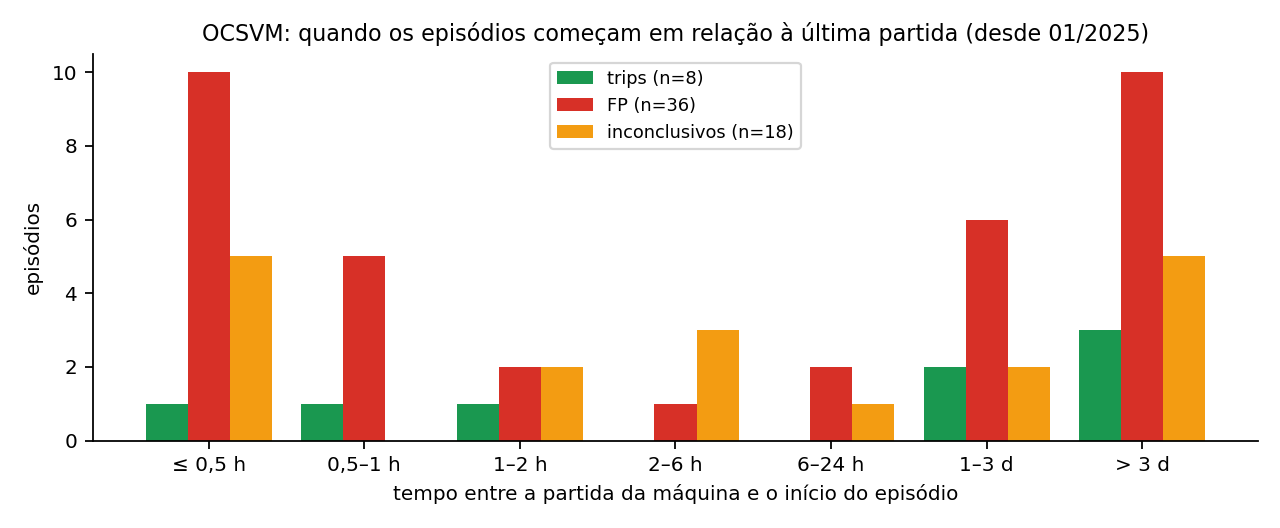
\includegraphics[width=0.85\textwidth]{partida.png}
\caption{Tempo entre a última partida e o início de cada alerta, desde 01/2025: trips (verde), alertas sem trip
(vermelho) e alertas seguidos de parada (laranja).}
\label{fig:partida}
\end{figure}

%=====================================================================
\section{O que pedimos}
%=====================================================================

Em ordem de importância. Respostas parciais já ajudam, e ``não sei'' também é uma resposta útil.

\begin{table}[H]
\centering\small
\begin{tabular}{>{\raggedright\arraybackslash}p{0.4cm} >{\raggedright\arraybackslash}p{5.2cm}
                >{\raggedright\arraybackslash}p{3cm} >{\raggedright\arraybackslash}p{5.9cm}}
\toprule
 & o que & período & para que serve \\
\midrule
1 & \textbf{Planilha anexa}, abas 1 a 4: tipo de cada partida, causa das paradas, o que aconteceu nos alertas sem
trip, perguntas pontuais & 07/2024 a 04/2026 & Explicar cada alerta, transformar ``inconclusivos'' em acerto ou erro e
separar partidas normais das problemáticas \\
2 & \textbf{Dados novos}: os mesmos sinais (resolução de 30~s), o catálogo de alarmes e a lista de trips e paradas &
21/04/2026 até hoje & Testar o modelo em eventos que ele nunca viu. É o único teste limpo de tudo o que foi
ajustado \\
3 & \textbf{Registro de partidas e paradas} (livro de turno ou sistema), com motivo & 07/2024 até hoje & Confirmar
e completar a aba 1 sem depender da memória da equipe \\
4 & \textbf{Ordens de serviço e notas de manutenção} da TC-33003A: mancais, vibração, óleo lubrificante, gás
combustível, motor de partida e instrumentação & 07/2024 até hoje & Explicar a série de vibração de 01--02/2026 e os
alertas sem causa \\
5 & \textbf{Histórico de configuração dos alarmes} (setpoints, habilitação, supressão) e \textbf{status completo}
(reconhecimento, retorno ao normal) & 07/2024 até hoje & Entender por que \tg{PI_6240319_AL} parou em 27/02/2026 e
por que \tg{PAL_6240315} recorre tanto \\
6 & \textbf{Eventos do sistema de aquisição}: falhas de comunicação, reinícios, manutenção de instrumentos &
07/2024 até hoje & Separar eventos de instrumentação (rajadas, ``Comm Fail'') de eventos de processo \\
7 & \textbf{Unidades de engenharia} dos tags e \tg{PI_0308} na resolução nativa & -- & Leitura física dos alertas;
cerca de 13\% do \tg{PI_0308} chega interpolado \\
\bottomrule
\end{tabular}
\end{table}

\subsection{A planilha anexa}

\begin{itemize}
  \item \textbf{Instruções:} como preencher.
  \item \textbf{1. Partidas (83):} as vezes em que a máquina voltou a operar, com quantas horas ficou parada antes.
        Pedimos o tipo da partida: normal após parada programada, após trip, após manutenção, teste ou partida
        abortada, ou não sei.
  \item \textbf{2. Paradas (31):} paradas sem alarme crítico. Pedimos se foram programadas, operacionais sem falha
        ou falha de equipamento. Substitui a planilha de 15/10, que não chegou a ser enviada.
  \item \textbf{3. Alertas sem trip (41):} cada alerta com os sinais que acenderam e os alarmes das 24~h anteriores.
        Pedimos o que estava acontecendo: manobra ou intervenção, problema de instrumento, evento de processo sem
        falha, nada de anormal, ou não sei.
  \item \textbf{4. Perguntas pontuais (8):} vibração em 01--02/2026, \tg{PI_6240319_AL}, \tg{PAL_6240315}, as 19
        rajadas de alarmes de temperatura, os 4 trechos de falha de comunicação, unidades e resolução do
        \tg{PI_0308}.
  \item \textbf{Trips curados (referência):} os 8 trips já reconhecidos, só para comparação.
\end{itemize}

As listas foram montadas a partir dos sinais, não de registros da operação. Os horários podem ter alguns minutos de
diferença e vêm em Brasília (UTC$-$3) e em UTC, que é o relógio dos dados. As abas não indicam o que o modelo acha de
cada linha, para não influenciar a resposta.

%=====================================================================
\section{O que faremos com cada resposta}
%=====================================================================

\begin{itemize}
  \item \textbf{Tipo de partida:} verificar se os alertas pós-partida sem trip vêm de partidas normais, e os trips de
        partidas após problema ou manutenção. Se sim, a informação vira um canal do modelo. Se não, ensinamos ao
        modelo o regime das primeiras horas de operação, que hoje ele não conhece.
  \item \textbf{Alertas classificados:} separar os alertas de instrumento dos de processo. Os de instrumento podem ser
        filtrados com regra; os de processo sem falha medem o custo real do modelo.
  \item \textbf{Causa das paradas:} 25 alertas hoje são ``inconclusivos'' porque foram seguidos de parada sem causa
        conhecida. Cada um vira acerto ou erro.
  \item \textbf{Alarmes e manutenção:} revalidar o canal de alarmes depois de 27/02/2026 e decidir se
        \tg{PAL_6240315} deve continuar nele.
  \item \textbf{Dados novos:} rodar o modelo atual, congelado, nos meses depois de 20/04/2026 e medir acertos e
        alertas falsos em eventos que nunca foram usados para ajustá-lo.
\end{itemize}

Todo teste com essas informações é registrado antes de rodar (o que se espera e o critério de aceite), para que a
conclusão não seja ajustada ao resultado.

\end{document}
